\chapter{Eksperymentalny algorytm klasyfikatora \emph{fingerprintów}}

\section{Motywacja}
Wcześniej w~niniejszej pracy zostało zaznaczone, że \emph{fingerprint} może być
bardziej unikalny kosztem jego stabilności i~odwrotnie. Aby zgrupować kolejne
\emph{fingerprinty} tej samej przeglądarki internetowej, których różnice
wynikają z~naturalnych przemian tej przeglądarki (np. aktualizacja), możemy użyć
klasyfikatora opartego na odpowiednim algorytmie. Tę relację przedstawia Rys. 7.
Dzięki takiemu rozwiązaniu jesteśmy w~stanie zachować wiarygodny wskaźnik
entropii, używając średnio bardziej unikalnych \emph{fingerprintów} o~mniejszej
stabilności.

Podobne (bardziej ograniczone) rozwiązanie zastosował Eckersley w~swojej pracy,
w~której po raz pierwszy opisał \emph{fingerprinting} przeglądarek internetowych
\cite[s. 13]{eckersley2010unique}.

\begin{figure}
	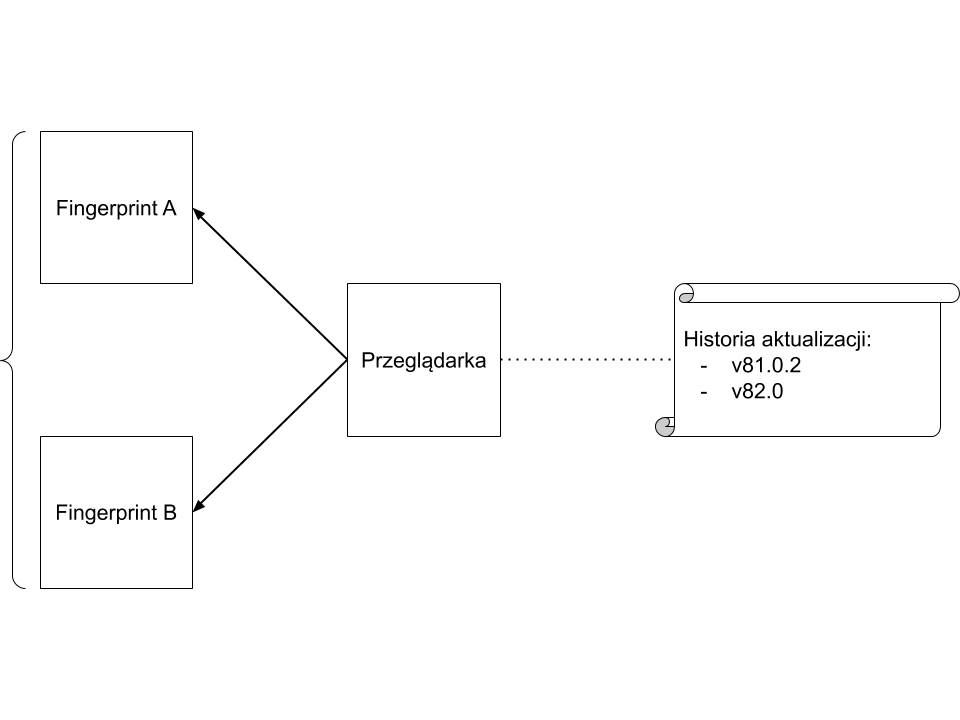
\includegraphics[width=\textwidth,keepaspectratio]{img/09}
	\source{Diagram przygotowany przez autora niniejszej pracy}
	\caption{Relacja \emph{fingerprint}--przeglądarka}
\end{figure}

\section{Opis algorytmu}
Aby zgrupować kolejne, podobne do siebie \emph{fingerprinty} należy wyznaczyć
podobieństwo każdego nowego \emph{fingerprintu} do wszystkich przechowywanych
i~utożsamić go z~tym, do którego jest najbardziej podobny (powyżej pewnej
wartości podobieństwa). Można to zrobić na parę sposobów. Jednym
z~najsensowniejszych rozwiązań wydaje się podejście, w~którym określa się
podobieństwo cech (komponentów) \emph{fingerprintu}, pomiędzy którymi istnieje
relacja większości (częściowy porządek). Tak można porównywać na przykład
nagłówki User-Agent (zawiera w~sobie wersję oprogramowania) jako komponent dwóch
porównywanych \emph{fingerprintów}. Z~tych porównań można wnioskować o~ogólnym
podobieństwie dwóch \emph{fingerprintów}.

Określanie podobieństwa komponentów, które bezpośrednio lub pośrednio wynikają
z~np. parametrów sprzętowych urządzenia (na przykład \emph{fingerprint} elementu
\texttt{canvas}), wydaje się bezcelowe. Ich wartość jest zwykle stała
i~należałoby zastanowić się nad istnieniem częściowego porządku w~takim zbiorze.
Jednakże ta niezmienność i~dalej porównywanie tych komponentów na zasadzie
równoważności może być przydatne w~szacowaniu, w~jakim stopniu ogólne
podobieństwo jest wiarygodne.

Metryką określającą podobieństwo do siebie dwóch komponentów będzie odległość
Levenshteina, która jest powszechnie stosowaną miarą odmienności skończonych
ciągów znaków.

\subsection{Odległość Levenshteina}
Algorytmy wyznaczające odległość Levenshteina nie są na tyle popularne, aby
znalazły one swoją implementację w~bibliotekach standardowych większości
popularnych języków oprogramowania. Z~tego względu autor niniejszej pracy
zdecydował się na własnoręczną implementację.

\subsubsection{Definicja}
Odległość Levenshteina pomiędzy dwoma łańcuchami znaków \(a\) i~\(b\)
o~długościach odpowiednio \(i\) i~\(j\), zdefiniowana jest jako
\begin{displaymath}
	\operatorname{ol}(i,j)=
	\begin{cases}
		\max(i,j)                    & \text{jeśli }\min(i,j)=0,  \\
		\min
		\begin{cases}
		\operatorname{ol}(i-1,j)+1 \\
		\operatorname{ol}(i,j-1)+1 \\
		\operatorname{ol}(i-1,j-1)   & \text{jeśli }a_i=b_j,      \\
		\operatorname{ol}(i-1,j-1)+1 & \text{jeśli }a_i \neq b_j. 
	\end{cases} & \text{w innym przypadku}.
	\end{cases}
\end{displaymath}

\subsubsection{Algorytm Wagnera--Fischera}
Bezpośrednia implementacja (z definicji) algorytmu wyznaczającego odległość
Levenshteina ma zasadniczy problem: tak zaimplementowany algorytm będzie działać
w~czasie ponadwielomianowym. Aby się o~tym przekonać, wystarczy narysować drzewo
wywołań rekurencyjnych i~zauważyć, że kolejne wywołania nie są rozłączne (nie
jest to oczywiście formalny dowód). Wyznaczanie odległości Levenshteina cechuje
własność optymalnej podstruktury i~bazując na programowaniu dynamicznym, można
znaleźć algorytm działający w~czasie wielomianowym.

Jednym z~takich algorytmów jest algorytm Wagnera--Fischera\footnote{Algorytm
	miał wielu wynalazców. Nazwa ,,Wagnera--Fischera'' powinna być traktowana
	jedynie jako zwyczajowa:
	https://en.wikipedia.org/wiki/Wagner-Fischer\_algorithm\#History} (Algorytm
2) \cite{wagner1974string}. Implementacja 4 przedstawia implementację
algorytmu Wagnera--Fischera. Implementacja 5 jest optymalnym wariantem tego
algorytmu (biorąc pod uwagę zużycie pamięci; Implementacja 4 zużywa
kwadratową ilość pamięci a~Implementacja 5 liniową). Taki wariant jest
stosowany później w~algorytmie klasyfikatora.

\begin{algorithm}
	\SetAlgoVlined
	\SetAlgoCaptionSeparator{.}
	\SetKwInOut{Input}{Dane}
	\SetKwInOut{Output}{Wynik}
	\SetKwData{VarM}{m}
	\SetKwData{VarN}{n}
	\SetKwData{VarC}{c}
	\SetKwArray{VarA}{a}
	\SetKwArray{VarB}{b}
	\SetKwArray{VarD}{d}
	\SetKwArray{VarE}{}
	\SetKwFunction{Minimum}{minimum}
	\BlankLine
	\Input{ciągi znaków \VarA i~\VarB o~długościach odpowiednio \VarM i~\VarN}
	\Output{odległość Levenshteina}
	\BlankLine
	\VarD $\leftarrow$ \VarE{$0 \dots$ \VarM, $0 \dots$ \VarN}\;
	\For{$i \leftarrow 1$ \KwTo \VarM}{
		\VarD{$i$, $0$} $\leftarrow i$\;
	}
	\For{$j \leftarrow 1$ \KwTo \VarN}{
		\VarD{$0$, $j$} $\leftarrow j$\;
	}
	\For{$j \leftarrow 1$ \KwTo \VarN}{
		\For{$i \leftarrow 1$ \KwTo \VarM}{
			\eIf{\VarA{$i - 1$} $=$ \VarB{$j - 1$}}{
				\VarC $\leftarrow 0$\;
				}{
				\VarC $\leftarrow 1$\;
			}
			\VarD{$i$, $j$} $\leftarrow$ \Minimum{\VarD{$i - 1$, $j$} $+$ $1$, \VarD{$i$, $j - 1$} $+$ $1$, \VarD{$i - 1$, $j - 1$} $+$ \VarC}\;
		}
	}
	\Return{\VarD{\VarM, \VarN}}\;
	\caption{Algorytm Wagnera--Fischera}
\end{algorithm}

\lstinputlisting[float,language=Go,caption=Algorytm Wagnera--Fischera w~Go,firstline=18,lastline=44,tabsize=4]{go/levenshtein.go}

\lstinputlisting[float,language=Go,caption=Algorytm Wagnera--Fischera w~Go (liniowa pamięć),firstline=46,lastline=74,tabsize=4]{go/levenshtein.go}

\section{Pseudokod}
Algorytm 3 przedstawia pseudokod proponowanego algorytmu klasyfikatora
\emph{fingerprintów}. Funkcja \texttt{hardwareRelatedCompatibility} określa
równoważność komponentów mających binarną lub liczbową reprezentację (w tym
wcześniej omawianych, teoretycznie niezmiennych komponentów). Funkcja
\texttt{similarity} bazując na odległości Levenshteina, określa wzajemne
podobieństwo reszty komponentów. Implementacja 6 przedstawia implementację tego
algorytmu w~Go.

% [x] osCpu
% [x] languages
% [ ] colorDepth
% [ ] deviceMemory
% [ ] screenResolution
% [ ] availableScreenResolution
% [ ] hardwareConcurrency
% [ ] timezoneOffset
% [x] timezone
% [ ] sessionStorage
% [ ] localStorage
% [ ] indexedDB
% [ ] openDatabase
% [x] cpuClass
% [x] platform
% [x] plugins
% [ ] canvas
% [ ] touchSupport
% [x] fonts
% [ ] audio
% [ ] pluginsSupport
% [x] productSub
% [ ] emptyEvalLength
% [ ] errorFF
% [x] vendor
% [ ] chrome
% [ ] cookiesEnabled

\begin{algorithm}
	\SetAlgoVlined
	\SetAlgoCaptionSeparator{.}
	\SetKwInOut{Input}{Dane}
	\SetKwInOut{Output}{Wynik}
	\SetKwData{VarF}{f}
	\SetKwData{VarG}{g}
	\SetKwData{VarMax}{max}
	\SetKwData{VarRatio}{ratio}
	\SetKwData{VarCandidate}{candidate}
	\SetKwData{SetG}{G}
	\SetKwFunction{HardwareRelatedCompatibility}{hardwareRelatedCompatibility}
	\SetKwFunction{Continue}{continue}
	\SetKwFunction{Similarity}{similarity}
	\SetKw{Null}{NULL}
	\BlankLine
	\Input{Zbiór \emph{fingerprintów} \SetG i~\emph{fingerprint} \VarF}
	\Output{\emph{fingerprint}, do którego \VarF jest najbardziej podobny, jeśli istnieje}
	\BlankLine
	\VarMax $\leftarrow 0$\;
	\ForEach{\VarG $\in$ \SetG}{
		\If{\HardwareRelatedCompatibility{\VarF, \VarG} $< \alpha$}{
			\Continue\;
		}
		\BlankLine
		\VarRatio $\leftarrow$ \Similarity{\VarF, \VarG}\;
		\BlankLine
		\If{\VarRatio $>$ \VarMax}{
			\VarMax $\leftarrow$ \VarRatio\;
			\VarCandidate $\leftarrow$ \VarG\;
		}
	}
	\If{\VarMax $\ge \beta$}{
		\Return{\VarCandidate}\;
	}
	\Return{\Null}\;
	\caption{Eksperymentalny klasyfikator}
\end{algorithm}

\lstinputlisting[float,language=Go,caption=Eksperymentalny klasyfikator w~Go,firstline=579,lastline=604,tabsize=4]{go/classifier.go}

\section{Ocena złożoności czasowej i~pamięciowej}
Załóżmy: \texttt{hardwareRelatedCompatibility} działa w~czasie stałym. Zgodnie
z~wcześniejszym ustaleniami \texttt{similarity} powinna działać w~czasie co
najwyżej kwadratowym, proporcjonalnym do długości \emph{fingerprintu} (algorytm
Wagnera--Fischera działa w~czasie \(\Theta(mn)\), gdzie \(m\) i~\(n\) to
długości porównywanych ciągów). Warto jednak zauważyć, że długość
\emph{fingerprintu} jest stała. Proponowany algorytm przegląda wszystkie
zapisane wcześniej \emph{fingerprinty} i~dla każdego obrotu wykonuje stałą
pracę. Możemy zatem stwierdzić, że proponowany algorytm działa w~czasie
liniowym.

Mając na uwadze rozważania z~poprzedniego akapitu, możemy także stwierdzić, że
pamięć używana przez proponowany algorytm jest stała.

\section{Ocena efektywności}

\subsection{Opis utworzonego rozwiązania}
W celu zbadania efektywności proponowanego algorytmu utworzono system złożony
z~dokumentowej bazy danych przechowującej zbierane przez aplikację serwera
(implementującego Algorytm 3; Implementacja 6) \emph{fingerprinty}, który
serwował także uruchamiany po stronie przeglądarki klienta (ofiary) skrypt je
generujący. Komponenty używane do generowania \emph{fingerprintu} przedstawiają
Tab. 1 i~Tab. 2. Listing kodu serwera i~kodu uruchamianego po stronie klienta
dostępny jest w~załącznikach do pracy.

\begin{table}
	\centering
	\caption{Komponenty używane w~implementacji klasyfikatora}
	\begin{tabular}{|l|c|}
		\hline
		Komponent                                   & Związany z~konfiguracją sprzętową? \\
		\hline
		\emph{fingerprint} elementu \texttt{canvas} & Tak                                    \\
		\texttt{Error.prototype.toSource()}         & Nie                                    \\
		\texttt{eval.toString().length}             & Nie                                    \\
		\texttt{navigator.browserLanguage}          & Nie                                    \\
		\texttt{navigator.cpuClass}                 & Tak                                    \\
		\texttt{navigator.deviceMemory}             & Tak                                    \\
		\texttt{navigator.hardwareConcurrency}      & Tak                                    \\
		\texttt{navigator.language}                 & Nie                                    \\
		\texttt{navigator.languages}                & Nie                                    \\
		\texttt{navigator.maxTouchPoints}           & Tak                                    \\
		\texttt{navigator.oscpu}                    & Nie                                    \\
		\texttt{navigator.platform}                 & Nie                                    \\
		\texttt{navigator.plugins}                  & Nie                                    \\
		\texttt{navigator.productSub}               & Nie                                    \\
		\texttt{navigator.systemLanguage}           & Nie                                    \\
		\texttt{navigator.userLanguage}             & Nie                                    \\
		\texttt{navigator.vendor}                   & Nie                                    \\
		\texttt{TouchEvent}                         & Tak                                    \\
		\texttt{window.chrome}                      & Nie                                    \\
		\texttt{window.indexedDB}                   & Nie                                    \\
		\texttt{window.Intl.DateTimeFormat()}       & Nie                                    \\
		\texttt{window.localStorage}                & Nie                                    \\
		\texttt{window.OfflineAudioContext}         & Tak                                    \\
		\texttt{window.ontouchstart}                & Tak                                    \\
		\texttt{window.openDatabase}                & Nie                                    \\
		\texttt{window.screen.availHeight}          & Tak                                    \\
		\texttt{window.screen.availWidth}           & Tak                                    \\
		\texttt{window.screen.colorDepth}           & Tak                                    \\
		\hline
	\end{tabular}
\end{table}

\begin{table}
	\centering
	\caption{Komponenty używane w~implementacji klasyfikatora cd.}
	\begin{tabular}{|l|c|}
		\hline
		Komponent                                 & Związany z~konfiguracją sprzętową? \\
		\hline
		\texttt{window.screen.height}             & Tak                                    \\
		\texttt{window.screen.width}              & Tak                                    \\
		\texttt{window.sessionStorage}            & Nie                                    \\
		\texttt{window.webkitOfflineAudioContext} & Tak                                    \\
		Lista czcionek                            & Nie                                    \\
		Obsługa \emph{cookies}                   & Nie                                    \\
		Przesunięcie strefy czasowej             & Nie                                    \\
		\hline
	\end{tabular}
\end{table}

\subsection{Testy efektywności}
Po wejściu na stronę interfejs widoczny na Rys. 8 informował użytkownika o~tym,
czy \emph{fingerprint} jego przeglądarki/urządzenia znajduje się już w~bazie
danych, skrócie \emph{fingerprintu}, czasie wykonania skryptu i~zebranych
komponentach.

Krótkie (dobrowolne) testy przeprowadzone na grupie znajomych autora pokazały,
że prosta heurystyka bez problemu poradziła sobie z~unikalną identyfikacją
użytkowników, a~także identyfikacją pomiędzy normalnym trybem przeglądarki
a~tzw. trybem prywatnym (najnowsze wersje niektórych przeglądarek internetowych
fałszują wartości komponentów pomiędzy trybami---w domyśle w~celach ochrony
prywatności). Algorytm radził sobie często także w~unikalnej identyfikacji
użytkowników pomiędzy przeglądarkami zainstalowanymi na tym samym urządzeniu.

\begin{figure}
	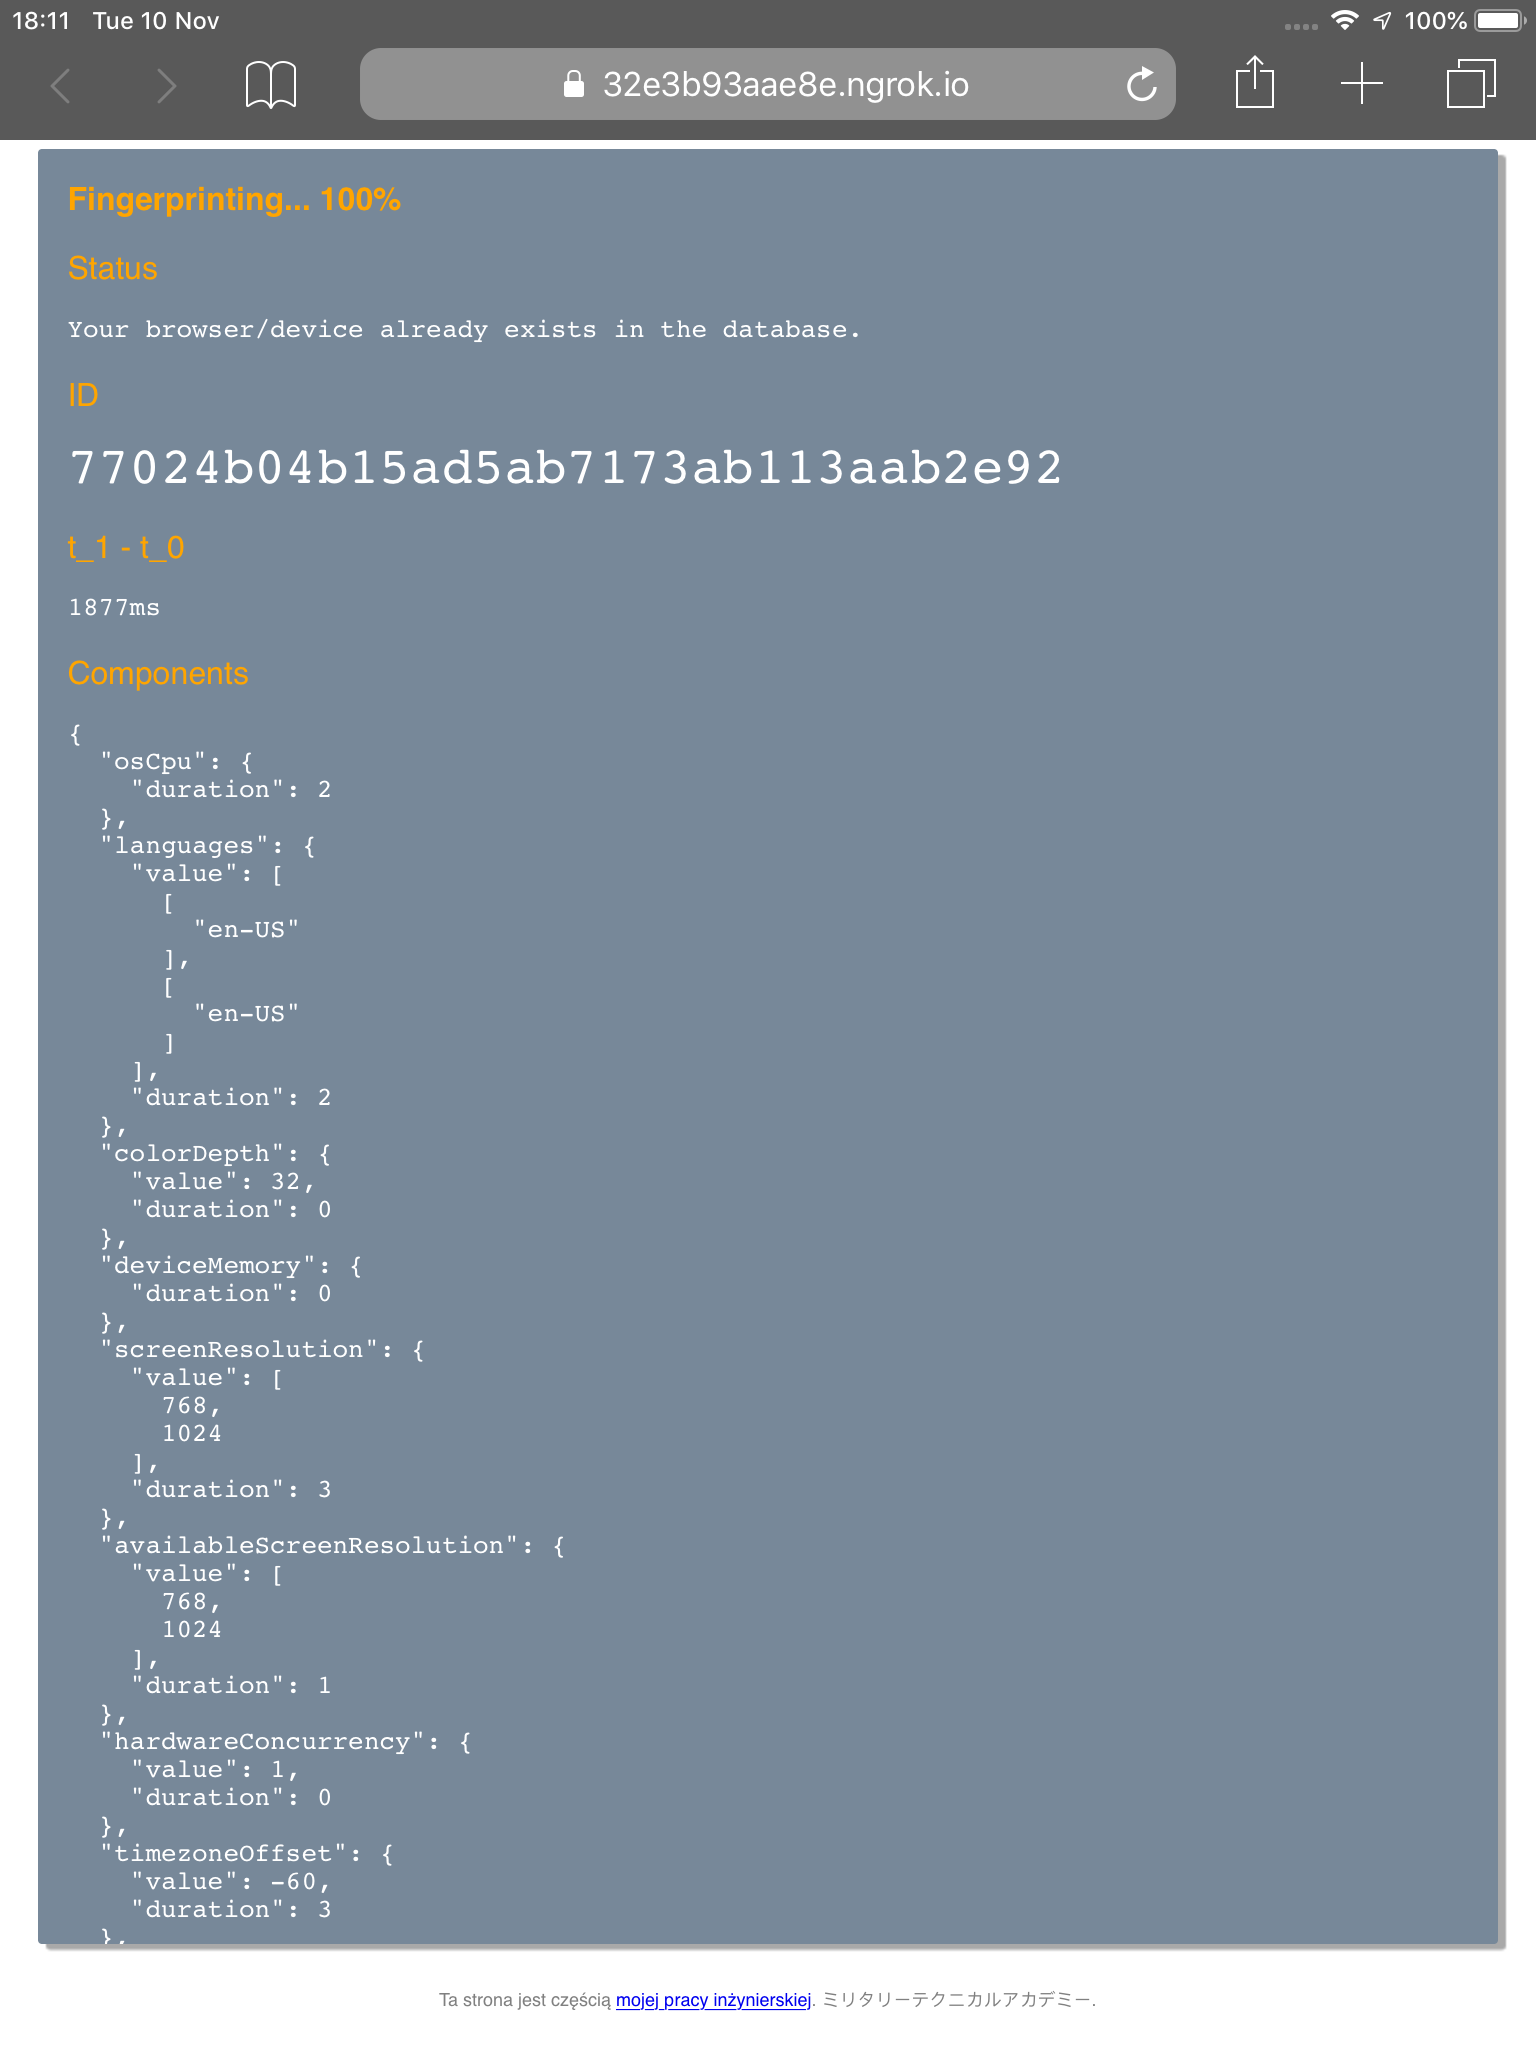
\includegraphics[width=\textwidth,keepaspectratio]{img/10}
	\source{Zrzut ekranu wykonany na urządzeniu Apple iPad Air}
	\caption{Interfejs aplikacji klienckiej eksperymentalnego klasyfikatora}
\end{figure}

\subsection{Wnioski}
Przeprowadzenie testu na większej grupie użytkowników pozwoliłoby określić
faktyczną skuteczność algorytmu. Pozwoliłoby określić procent poprawnych,
niezamierzonych i~nieutworzonych klasyfikacji, a~także oszacować teoretyczną
granicę entropii dla proponowanych komponentów. Taka analiza pokazałaby także
które komponenty można byłoby odrzucić, a~które dodać. W~przypadku
przeprowadzenia większego testu zastosowanie wyników analizy, jakie binarne
i~liczbowe źródła danych powinny mieć większą wagę (w przedstawionej
implementacji funkcja \texttt{hardwareRelatedCompatibility} traktuje
zgodność/niezgodność wszystkich komponentów tak samo; w~domyśle komponenty
związane z~konfiguracją sprzętową powinny mieć większą wagę) mogłoby zredukować
liczbę fałszywie dodatnich oraz fałszywie ujemnych wyników klasyfikacji.
Istnieje także możliwość, że zaproponowany heurystyczny algorytm okaże się mniej
wydajny od np. zastosowania metod uczenia maszynowego do klasyfikacji
\emph{fingerprintów}. Podsumowując: wyniki przeprowadzonego testu wskazują na
spory potencjał w~stosowaniu takich rozwiązań jak klasyfikatory. Niestety nie
jest to także dobra wiadomość dla prywatności typowych użytkowników Internetu.
